\subsection{周波数応答}

制御系の信号は、まず時刻を横軸にした時間波形として観測される。ステップ応答の時間波形は、出力がどれくらい速く目標値へ近づき、どれくらい行き過ぎ、どの程度で整定するかを直接示す。これは時間領域の仕様として重要である。しかし、同じ時間波形だけでは、ゆっくりした目標値変化、急な立上り、測定ノイズ、機械共振、電源リップル、サンプリングに由来する周期的変動が、それぞれ制御系をどのように通過したかを分離しにくい。急な目標値変更で大きなオーバーシュートが生じる場合も、立上りを作る速い変化が制御対象の帯域制限や共振でどう変形されたかは、時間波形だけからは判定しにくい。

この分離を行うために、時間波形を正弦波または複素指数関数の成分へ分解して考える。周期信号を離散的な周波数成分の和として表すときはフーリエ級数を用いる。非周期信号を広い時間範囲で扱い、適切な可積分性やエネルギー条件のもとで連続的な周波数成分として表すときはフーリエ変換を用いる。これらは、時間信号にどの周波数成分がどれだけ含まれるかを記述する方法である。

ラプラス変換はフーリエ級数やフーリエ変換と役割が異なる。ラプラス変換では、複素変数 $s=\sigma+j\omega$ と収束域を用いて、初期条件、過渡応答、極、零点、安定性、伝達関数を同じ枠で扱う。フーリエ変換がラプラス変換の虚軸上の値と形式的に結びつく場合はあるが、成立条件と目的は単に同じではない。周波数応答は、フーリエ解析で信号を正弦波成分へ分け、その各成分が安定な線形時不変系を通過した後の振幅比と位相差を、ラプラス変換で得た伝達関数の虚軸上の値から評価する手順である。

\subsubsection{方形波部分和による周波数成分の解釈}

正弦波成分への分解は、正弦波だけが現実の信号であるという仮定ではない。周期信号の多くは、基本周波数とその整数倍の正弦波成分の和として表せる。したがって、各周波数成分に対するゲインと位相が分かれば、複雑な周期信号が制御系を通った後にどの成分を保ち、どの成分を遅らせ、どの成分を減衰するかを整理できる。方形波はこの関係を確認しやすい標準例である。

周期 $2\pi$ の方形波
\begin{equation}
  q(\theta)=
  \begin{cases}
    1, & 0<\theta<\pi,\\
    -1, & \pi<\theta<2\pi
  \end{cases}
\end{equation}
を考える。ただし $q(\theta+2\pi)=q(\theta)$ とする。この奇関数のフーリエ級数は奇数次の正弦波だけを含み、奇数 $N$ までで打ち切った部分和を
\begin{equation}
  q_N(\theta)=
  \frac{4}{\pi}\sum_{\substack{k=1\\k\ \mathrm{odd}}}^{N}
  \frac{\sin k\theta}{k}
  \label{eq:square-wave-fourier-partial}
\end{equation}
と書く。

\begin{figure}[tb]
\centering
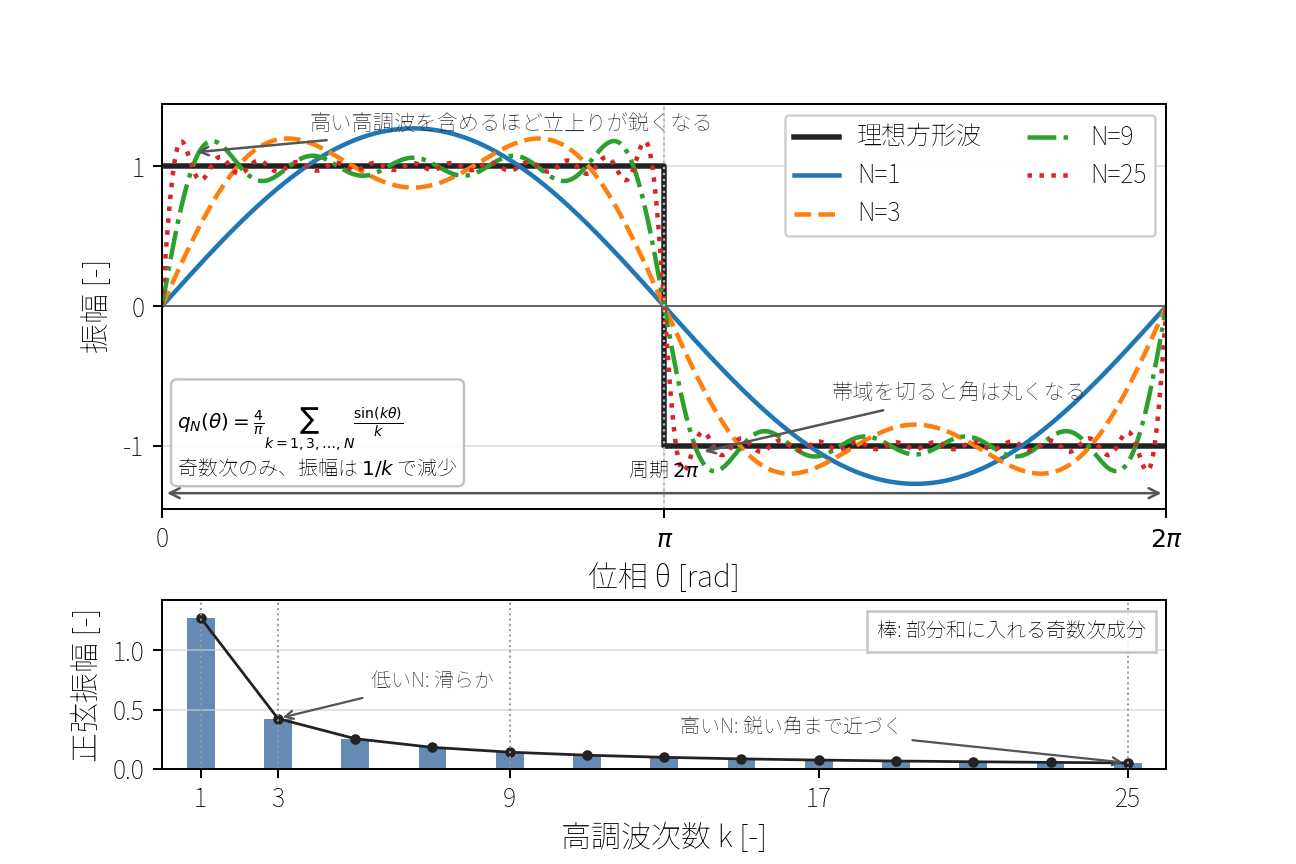
\includegraphics[width=0.88\linewidth,bb=0 0 1296 864]{figures/fourier_square_partial_sums.png}
\caption{周期 $2\pi$、振幅 $\pm1$ に正規化した方形波と、奇数次高調波 $k=1,3,\ldots,N$ だけを $N=1,3,9,25$ で打ち切ったフーリエ部分和。高い奇数次高調波ほど不連続点近傍の鋭い立上りを作るため、帯域制限をもつ制御対象や閉ループでは方形波指令や急な外乱が丸められ、帯域付近の位相遅れや共振が過渡応答として現れやすい。}
\label{fig:fourier-square-partial-sums}
\end{figure}

図\ref{fig:fourier-square-partial-sums} では、$N$ を増やすほど平坦部が $\pm1$ に近づき、不連続点の近くで急な変化が作られる。$N=1$ は基本波だけなので角は再現されず、波形全体が滑らかな正弦波として残る。$N=3$ や $N=9$ では低次の奇数次高調波が平坦部と立上りを作り始め、$N=25$ では高次成分によって立上りがさらに鋭くなる一方、不連続点近傍には部分和特有の振動が集中する。したがって理想的な方形波には、任意に高い奇数次高調波が必要である。制御対象や閉ループが $k=9$ 以上の成分をほとんど通過させないなら、出力は高次部分和ではなく低次部分和に近い形になり、方形波指令や急な外乱の角は有限の傾きをもつ丸い立上りへ変わる。帯域付近に大きな位相遅れや共振があれば、その丸められた立上りの後に遅れ、行き過ぎ、残留振動が時間波形として現れる。

\subsubsection{正弦波定常応答と伝達関数の虚軸評価}

線形時不変系では、各正弦波成分を個別に評価できる。安定な線形時不変系、または対象とする初期条件で過渡成分が減衰する線形時不変系に正弦波を入れると、過渡成分が消えた後の出力も同じ周波数の正弦波になる。入力を $u(t)=A\sin \omega t$ とする。ただし $A$ は振幅、$\omega\,[\mathrm{rad/s}]$ は角周波数である。このとき出力は
\begin{equation}
  y(t)=A\abs{G(j\omega)}\sin\{\omega t+\angle G(j\omega)\}
\end{equation}
で表せる。$G(j\omega)$ は伝達関数 $G(s)$ に $s=j\omega$ を代入したものである。安定で虚軸上の評価が収束する系では、$G(j\omega)$ が角周波数 $\omega$ の成分に対する複素倍率を与える。絶対値 $\abs{G(j\omega)}$ が入力振幅に対する出力振幅の比、偏角 $\angle G(j\omega)$ が入力正弦波に対する出力正弦波の位相差を表す。

一次遅れ $G(s)=K/(\tau s+1)$ について、ここでは $K>0$ とする。このとき
\begin{align}
  \abs{G(j\omega)}&=\frac{K}{\sqrt{1+(\tau\omega)^2}},\\
  \angle G(j\omega)&=-\tan^{-1}(\tau\omega).
\end{align}
低周波では入力がゆっくり変化するため出力はほぼ追従し、高周波では対象の応答遅れによりゲインが低下し位相が遅れる。時定数 $\tau$ が大きいほど、同じ $\omega$ でも $\tau\omega$ が大きくなるため、振幅低下と位相遅れが低い周波数から現れる。周波数応答は、目標値、ノイズ、振動成分が制御系を通過する際の振幅比と位相差を表す。

この情報は安定性、ロバスト性、ノイズ感度の評価に直結する。フィードバック系の閉ループ極は特性方程式で決まるが、開ループ $L(j\omega)$ のゲインと位相を周波数ごとに調べると、ゲイン増加、むだ時間、未モデル化共振、追加の位相遅れがゲイン余裕・位相余裕をどの帯域で減らすかを特定できる。一方、センサノイズは相補感度関数や制御入力の大きさを通じて出力変動、追従精度、アクチュエータ飽和余裕を制限する性能要因であり、飽和などの非線形実装効果を介する場合を除けば、線形解析上は閉ループ極を直接に不安定側へ動かさない。したがって、周波数応答は時間応答の代替ではなく、時間波形で観察した振動やオーバーシュートを、ゲイン余裕、位相余裕、帯域幅、感度関数、相補感度関数として定量化するための橋渡しである。

\subsection{ボード線図}

ボード線図は、横軸を対数目盛の角周波数 $\omega$ とし、上段にゲイン $20\log_{10}\abs{G(j\omega)}$、下段に位相 $\angle G(j\omega)$ を描く図である。ゲインを dB で表すと、伝達関数の積がゲイン線図では和になる。したがって
\begin{equation}
  G(s)=K\frac{(1+T_1s)(1+T_2s)}{s(1+\tau_1s)(1+\tau_2s)}
\end{equation}
のような形は、定数ゲイン、零点、積分器、一次遅れの寄与へ分解できる。

\subsubsection{因子分解によるボード線図の漸近作図}

漸近作図の目的は、厳密な数値計算を置き換えることではなく、どの周波数帯でどの因子が支配的かを図上で把握することである。ここでは各因子が無次元になるように正規化し、折点周波数を $\omega_b\,[\mathrm{rad/s}]$ と書く。1 decade は角周波数が 10 倍になる区間であり、ゲインの傾きは $\mathrm{dB/dec}$ で表す。

定数ゲイン $K$ は
\begin{equation}
  20\log_{10}\abs{K}
\end{equation}
だけゲイン線図を上下に移動させる。$K>0$ なら位相は $0^\circ$、$K<0$ なら全周波数で $180^\circ$ を加える。積分器と微分器は $s^q$ とまとめて書ける。係数側に必要な単位を含め、原点因子の周波数依存だけを評価するときは、基準角周波数 $\omega_0=1\,\mathrm{rad/s}$ で割って無次元化しておく。$q$ が正なら $q$ 個の微分器、負なら $-q$ 個の積分器であり、
\begin{align}
  20\log_{10}\abs{\left(\frac{j\omega}{\omega_0}\right)^q}
    &=20q\log_{10}\frac{\omega}{\omega_0},\\
  \angle (j\omega)^q
    &=90q^\circ
\end{align}
である。したがってゲイン傾きは $20q\,\mathrm{dB/dec}$ で、$1/s$ は $-20\,\mathrm{dB/dec}$ と $-90^\circ$、$s$ は $+20\,\mathrm{dB/dec}$ と $+90^\circ$ を与える。

左半平面にある実零点は
\begin{equation}
  F_z(s)=1+\frac{s}{\omega_z}
\end{equation}
と書ける。この因子の厳密なゲインと位相は
\begin{align}
  20\log_{10}\abs{F_z(j\omega)}
    &=10\log_{10}\left\{1+\left(\frac{\omega}{\omega_z}\right)^2\right\},\\
  \angle F_z(j\omega)
    &=\tan^{-1}\frac{\omega}{\omega_z}
\end{align}
である。$\omega\ll\omega_z$ では $F_z(j\omega)\simeq1$ なので $0\,\mathrm{dB}$、$\omega\gg\omega_z$ では $\abs{F_z(j\omega)}\simeq\omega/\omega_z$ なので $+20\,\mathrm{dB/dec}$ になる。よって $\omega_z$ を折点として、ゲイン傾きを $20\,\mathrm{dB/dec}$ 増やす。位相は $0^\circ$ から $+90^\circ$ へ移り、概略作図では $0.1\omega_z$ から $10\omega_z$ までを直線でつないで、$\omega_z$ で $+45^\circ$ と近似する。

左半平面の実極
\begin{equation}
  F_p(s)=\frac{1}{1+s/\omega_p}
\end{equation}
は実零点の逆数であるから、ゲインと位相の寄与は実零点の符号を反転したものになる。すなわち折点 $\omega_p$ を越えるとゲイン傾きは $20\,\mathrm{dB/dec}$ 減り、位相は $0^\circ$ から $-90^\circ$ へ移る。右半平面の実零点 $1-s/\omega_z$ や右半平面の実極 $1/(1-s/\omega_p)$ は、ゲイン線図の漸近線は左半平面因子と同じであるが、位相の符号が反対になる。したがって非最小位相零点や不安定極を含むときは、ゲインだけを見て位相余裕を推測してはならない。

二次因子は、減衰比 $\zeta>0$ と固有角周波数 $\omega_n$ を用いて
\begin{equation}
  F_2(s)=1+2\zeta\frac{s}{\omega_n}
    +\left(\frac{s}{\omega_n}\right)^2
\end{equation}
と書く。$0<\zeta<1$ なら共役複素極または零点に対応し、$\zeta\ge1$ なら二つの実一次因子へ分解してもよい。$r=\omega/\omega_n$ とおくと
\begin{align}
  F_2(j\omega)
    &=1-r^2+j2\zeta r,\\
  \abs{F_2(j\omega)}
    &=\sqrt{(1-r^2)^2+(2\zeta r)^2}.
\end{align}
二次零点 $F_2(s)$ は $\omega_n$ より十分低いところで $0\,\mathrm{dB}$、十分高いところで $+40\,\mathrm{dB/dec}$ となる。二次極 $1/F_2(s)$ は同じ折点で傾きが $40\,\mathrm{dB/dec}$ 減り、位相は $0^\circ$ から $-180^\circ$ へ移る。二次零点では位相の符号が逆になり、$0^\circ$ から $+180^\circ$ へ移る。$\omega=\omega_n$ では $F_2(j\omega_n)=j2\zeta$ なので、二次極の厳密なゲインは
\begin{equation}
  20\log_{10}\frac{1}{2\zeta}
  =-20\log_{10}(2\zeta)
\end{equation}
である。したがって小さい $\zeta$ では折点付近に山が現れ、二本の直線漸近線だけでは共振を評価できない。

一次因子の漸近線誤差は固定値として覚えられる。実零点で $x=\omega/\omega_z$ とおくと、ゲイン漸近線との差は
\begin{equation}
  e_z(x)=10\log_{10}(1+x^2)-\max\{0,20\log_{10}x\}
\end{equation}
である。折点 $x=1$ では $e_z(1)=10\log_{10}2\simeq3.01\,\mathrm{dB}$ であり、$x=0.1$ と $x=10$ では約 $0.043\,\mathrm{dB}$ まで小さくなる。実極の誤差は $-e_z(x)$ である。二次因子の折点誤差は $\zeta$ に依存し、二次極では $-20\log_{10}(2\zeta)$ が折点での厳密値になる。

以上を使うと、漸近作図の手順は明確になる。まず因子分解して折点周波数を小さい順に並べる。次に定数ゲインと原点因子から低周波側の高さと傾きを決める。折点を通過するたびに、実零点なら $+20$、実極なら $-20$、二次零点なら $+40$、二次極なら $-40$ を傾きに加える。位相線図は各因子の寄与を同じ周波数軸上で足し合わせる。最後に一次因子の折点で約 $3\,\mathrm{dB}$、二次因子では $\zeta$ に応じた誤差または共振ピークを補正して、漸近線と厳密線図のずれを評価する。

\begin{example}[積の形によるボード線図の漸近作図]
背景知識を必要としない例として、次の正規化された開ループを考える。$s$ と各折点周波数の単位は $\mathrm{rad/s}$ であり、原点因子も $\omega_0=1\,\mathrm{rad/s}$ で割って無次元化する。したがって定数 $5$ は無次元の倍率として扱える。
\begin{equation}
\begin{aligned}
  L(s)
  &=5\,\frac{1+s/\omega_z}{(s/\omega_0)(1+s/\omega_p)}\\
  &\quad{}\times
    \frac{1}{1+2\zeta s/\omega_n+(s/\omega_n)^2},\\
  \omega_0&=1\,\mathrm{rad/s},\quad
  \omega_p=0.2\,\mathrm{rad/s},\\
  \omega_z&=2\,\mathrm{rad/s},\quad
  \omega_n=20\,\mathrm{rad/s},\\
  \zeta&=0.5.
\end{aligned}
\end{equation}
因子は、定数ゲイン $5$、正規化積分器 $1/(s/\omega_0)$、実零点 $1+s/\omega_z$、実極 $1/(1+s/\omega_p)$、減衰比 $\zeta=0.5$ と固有角周波数 $20\,\mathrm{rad/s}$ の二次極である。折点は
\begin{equation}
  0.2,\qquad 2,\qquad 20
  \quad [\mathrm{rad/s}]
\end{equation}
の順に並ぶ。

低周波側の初期線分では定数ゲインが $20\log_{10}5\simeq14\,\mathrm{dB}$、正規化積分器が $-20\log_{10}(\omega/\omega_0)$、すなわち $-20\,\mathrm{dB/dec}$ の傾きを与える。この初期線分を $\omega=1\,\mathrm{rad/s}$ へ外挿した切片は約 $14\,\mathrm{dB}$ であるが、有効な区間は最初の折点 $0.2\,\mathrm{rad/s}$ より低い範囲である。たとえば $\omega=0.1\,\mathrm{rad/s}$ では積分器が $+20\,\mathrm{dB}$ を与え、初期漸近ゲインは約 $34\,\mathrm{dB}$ になる。その後、$\omega=0.2$ で実極により傾きは $-40\,\mathrm{dB/dec}$ へ変わるので、$\omega=1\,\mathrm{rad/s}$ の漸近値は実極の寄与 $-20\log_{10}(1/0.2)$ を含み約 $0\,\mathrm{dB}$ である。$\omega=2$ で実零点が加わり、傾きは $-20\,\mathrm{dB/dec}$ へ戻る。$\omega=20$ で二次極が加わり、傾きは $-60\,\mathrm{dB/dec}$ になる。

\begin{figure}[tb]
\centering
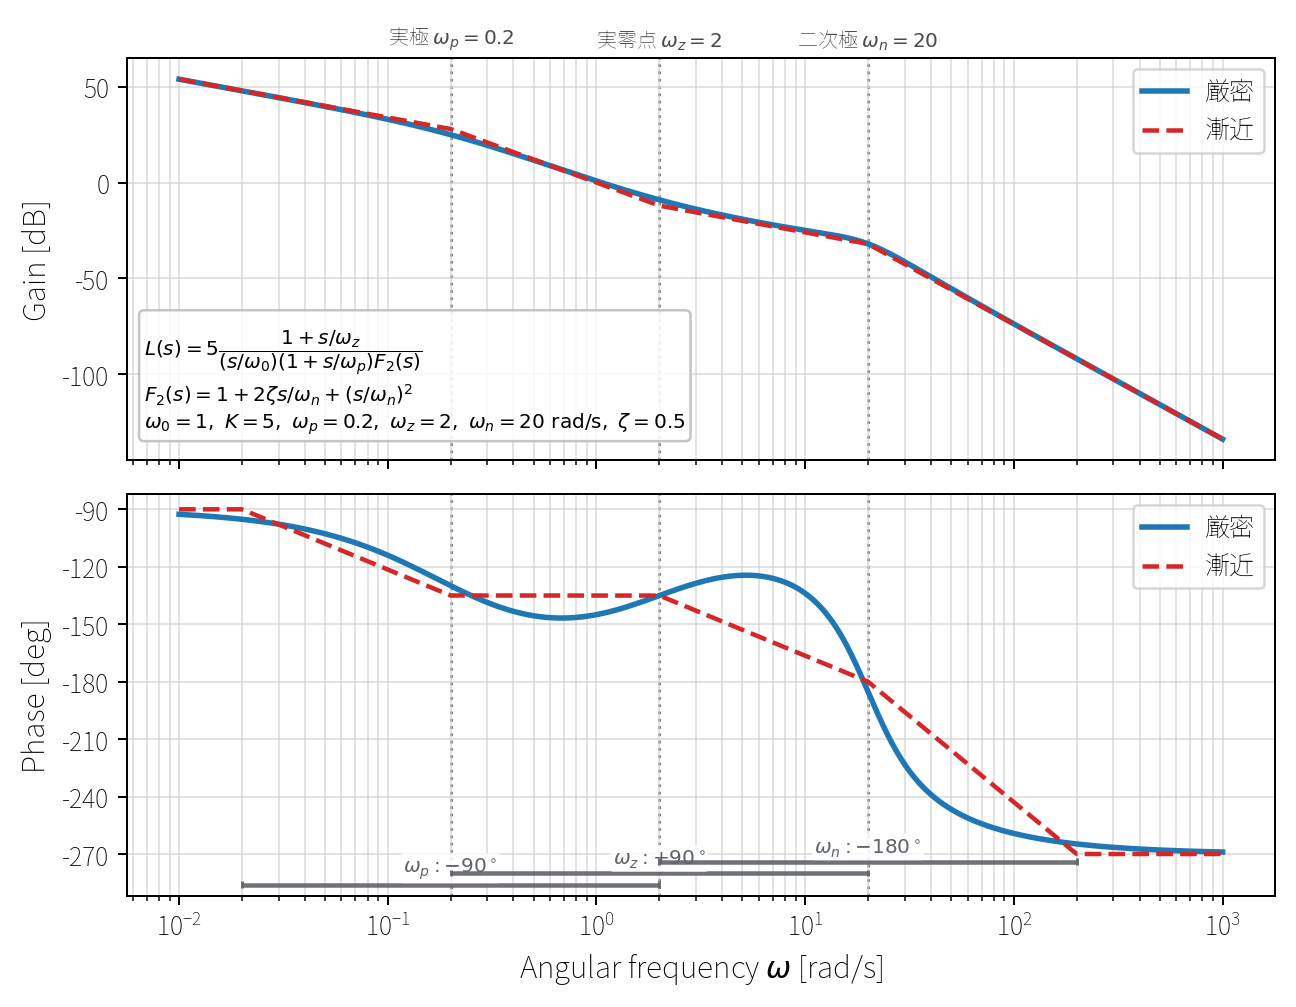
\includegraphics[width=0.88\linewidth,bb=0 0 1296 1007]{figures/bode_factor_example.png}
\caption{正規化された開ループ $L(s)$ のボード線図。$0.2\,\mathrm{rad/s}$ の実極でゲイン傾きが下がり、$2\,\mathrm{rad/s}$ の実零点で戻り、$20\,\mathrm{rad/s}$ の二次極でさらに低下する。破線の漸近線と実線の厳密線図を比べると、折点近傍の誤差と位相遷移を確認できる。}
\label{fig:bode-factor-example}
\end{figure}

位相は、正規化積分器の $-90^\circ$ から始める。実極 $1/(1+s/\omega_p)$ はおよそ $0.02$ から $2\,\mathrm{rad/s}$ の間でさらに $-90^\circ$ を加え、実零点 $1+s/\omega_z$ は $0.2$ から $20\,\mathrm{rad/s}$ の間で $+90^\circ$ を加える。二次極は $2$ から $200\,\mathrm{rad/s}$ 付近で $-180^\circ$ を加え、$\omega=20\,\mathrm{rad/s}$ では二次因子だけで $-90^\circ$ を与える。したがって高周波側の位相は、概略で
\begin{equation}
  -90^\circ-90^\circ+90^\circ-180^\circ=-270^\circ
\end{equation}
へ近づく。

折点近傍では直線だけを信用しすぎない。$\omega=0.2$ の実極は漸近線より約 $3\,\mathrm{dB}$ 低く、$\omega=2$ の実零点は約 $3\,\mathrm{dB}$ 高い。二次極は $\zeta=0.5$ なので $\omega=20$ での厳密な寄与が $20\log_{10}\{1/(2\zeta)\}=0\,\mathrm{dB}$ となり、折点そのものでは直線漸近線と一致する。しかし $\zeta$ がもっと小さければ、この周波数帯に共振の山が生じる。概略作図では、傾きの変化で全体の形を決め、折点誤差でゲイン値を補正する。
\end{example}

\subsubsection{余裕・交差周波数・帯域を仕様へ翻訳する}

本節では、設計仕様を開ループおよび閉ループの周波数応答指標として定義する。対象は単一入出力の単位負帰還系とし、開ループを
\begin{equation}
  L(s)=C(s)G(s)
\end{equation}
とおく。閉ループが安定で、評価する周波数で $L(j\omega)$ が定義できることを前提にする。開ループが右半平面極を持つ場合や交差周波数が複数ある場合には、余裕の値だけで安定性を断定せず、ナイキスト判別で閉ループ極の個数を確認する。

角周波数 $\omega$ の単位は $\mathrm{rad/s}$ である。周波数 $f\,[\mathrm{Hz}]$ で表すときは
\begin{equation}
  \omega=2\pi f
\end{equation}
を使う。ゲイン $\abs{L(j\omega)}$ は無次元の比であり、dB 表示では $20\log_{10}\abs{L(j\omega)}$ と書く。位相はラジアンまたは度で表す。むだ時間を含む式ではラジアンを用いる。

\begin{definition}[交差周波数と安定余裕]
ゲイン交差周波数 $\omega_{gc}$ は
\begin{equation}
  \abs{L(j\omega_{gc})}=1
\end{equation}
を満たす周波数である。これは dB 表示で $0\,\mathrm{dB}$ を横切る周波数である。位相交差周波数 $\omega_{pc}$ は、位相を連続につないで読んだとき
\begin{equation}
  \angle L(j\omega_{pc})=-\pi
  \qquad (-180^\circ)
\end{equation}
を満たす周波数である。ゲイン交差周波数での位相余裕を
\begin{equation}
  \phi_m=\pi+\angle L(j\omega_{gc})
\end{equation}
と定義する。度で表すなら $\phi_m=180^\circ+\angle L(j\omega_{gc})$ である。位相交差周波数でのゲイン余裕を
\begin{equation}
  g_m=\frac{1}{\abs{L(j\omega_{pc})}}
\end{equation}
と定義し、dB では
\begin{equation}
  G_{m,\mathrm{dB}}=20\log_{10}g_m
  =-20\log_{10}\abs{L(j\omega_{pc})}
\end{equation}
と表す。
\end{definition}

位相余裕の符号は、「あとどれだけ位相が遅れると $-180^\circ$ に達するか」を表すように取る。たとえば $\angle L(j\omega_{gc})=-135^\circ$ なら
\begin{equation}
  \phi_m=180^\circ-135^\circ=45^\circ
\end{equation}
である。正の位相余裕は、ゲイン交差周波数において位相が $-180^\circ$ に達していないことを示す。負の位相余裕は、同じ周波数で位相が $-180^\circ$ を越えていることを示す。ただし多重交差や不安定開ループ極がある場合には、この指標だけで閉ループ安定性を判定しない。

\begin{derivation}
ゲイン余裕が「何倍のゲイン増加に耐えるか」を表すことを式で見る。対象や制御器のゲインが見積もりより $k$ 倍になったとすると、開ループは $kL(s)$ になる。閉ループ特性方程式は
\begin{equation}
  1+kL(s)=0
\end{equation}
である。位相交差周波数では $L(j\omega_{pc})$ が負の実軸上にあり、
\begin{equation}
  L(j\omega_{pc})=-\abs{L(j\omega_{pc})}
\end{equation}
と書ける。境界的に $1+kL=0$ となる条件は
\begin{align}
  1-k\abs{L(j\omega_{pc})}&=0,\\
  k&=\frac{1}{\abs{L(j\omega_{pc})}}
\end{align}
である。したがって $g_m$ は、単純なゲイン増加に対する許容量を無次元倍率で表している。
\end{derivation}

位相余裕は、むだ時間の許容量の近似評価に用いられる。むだ時間 $\tau_d$ は開ループに $e^{-s\tau_d}$ を掛けるので、周波数 $\omega$ での追加位相遅れは
\begin{equation}
  \angle e^{-j\omega\tau_d}=-\omega\tau_d
\end{equation}
である。ゲイン交差周波数の近くで閉ループ安定性が決まると見なせるなら、許されるむだ時間の目安は
\begin{equation}
  \tau_{d,\max}\simeq\frac{\phi_m}{\omega_{gc}}
\end{equation}
となる。ただしこの式の $\phi_m$ はラジアンである。$\omega_{gc}$ が大きいほど、同一の位相余裕に対する許容むだ時間は短くなる。したがって、応答帯域を高く設定することと、むだ時間に対するロバスト性を増加させることは一般にトレードオフとなる。

閉ループの応答帯域は、相補感度
\begin{equation}
  T(s)=\frac{L(s)}{1+L(s)}
\end{equation}
の帯域幅により定義する。低周波で $T(0)\simeq 1$ なら、閉ループ帯域幅 $\omega_b$ は
\begin{equation}
  \abs{T(j\omega_b)}=\frac{1}{\sqrt{2}}\abs{T(0)}
\end{equation}
を初めて満たす周波数として定義する。これは低周波ゲインから
\begin{equation}
  20\log_{10}\frac{1}{\sqrt{2}}
  =-10\log_{10}2\simeq -3.01\,\mathrm{dB}
\end{equation}
下がる点である。$\omega_b$ より十分低い目標値成分はよく追従され、$\omega_b$ より高い成分は閉ループで減衰し始める。したがって、目標値や外乱の主成分を通したいなら $\omega_b$ をその周波数より上に置き、測定ノイズや未モデル化共振を入れたくないなら $\omega_b$ をそれらより十分低く置く。

一次閉ループ
\begin{equation}
  T_1(s)=\frac{1}{\tau_c s+1}
\end{equation}
では
\begin{equation}
  \abs{T_1(j\omega)}=\frac{1}{\sqrt{1+(\omega\tau_c)^2}}
\end{equation}
である。$\abs{T_1(j\omega_b)}=1/\sqrt{2}$ を代入すると
\begin{align}
  \frac{1}{\sqrt{1+(\omega_b\tau_c)^2}}&=\frac{1}{\sqrt{2}},\\
  1+(\omega_b\tau_c)^2&=2,\\
  \omega_b&=\frac{1}{\tau_c}
\end{align}
となる。一次応答の 10--90\% 立上り時間はおよそ $2.2\tau_c$、2\% 整定時間はおよそ $4\tau_c$ であるから、一次的に振る舞う閉ループでは
\begin{equation}
  t_r\simeq\frac{2.2}{\omega_b},
  \qquad
  T_s\simeq\frac{4}{\omega_b}
\end{equation}
という時間応答指標との近似対応が得られる。

閉ループゲインの最大値を共振ピークという。低周波ゲインが 1 に正規化された閉ループでは
\begin{equation}
  M_r=\max_{\omega\ge 0}\abs{T(j\omega)}
\end{equation}
で定義し、dB では $20\log_{10}M_r$ と表す。$M_r=1.3$ は約 $2.3\,\mathrm{dB}$ であり、対応する周波数成分の振幅比が 1.3 であることを表す。

二次標準閉ループ
\begin{equation}
  T_2(s)=\frac{\omega_n^2}{s^2+2\zeta\omega_n s+\omega_n^2}
\end{equation}
では、$r=\omega/\omega_n$ とおくと
\begin{align}
  \abs{T_2(j\omega)}^2
  &=\frac{\omega_n^4}{(\omega_n^2-\omega^2)^2+(2\zeta\omega_n\omega)^2}\\
  &=\frac{1}{(1-r^2)^2+(2\zeta r)^2}.
\end{align}
分母を
\begin{equation}
  D(r)=(1-r^2)^2+(2\zeta r)^2
  =1+(4\zeta^2-2)r^2+r^4
\end{equation}
とおく。共振ピークは $D(r)$ が最小になるところで生じるので、
\begin{align}
  \frac{\dd D}{\dd r}
  &=2(4\zeta^2-2)r+4r^3\\
  &=4r(r^2+2\zeta^2-1)
\end{align}
を 0 とおく。$r>0$ の解は
\begin{equation}
  r^2=1-2\zeta^2
\end{equation}
である。したがって $0<\zeta<1/\sqrt{2}$ のときだけ共振周波数
\begin{equation}
  \omega_r=\omega_n\sqrt{1-2\zeta^2}
\end{equation}
が存在し、そのピークは
\begin{equation}
  M_r=\frac{1}{2\zeta\sqrt{1-\zeta^2}}
\end{equation}
となる。$\zeta\ge 1/\sqrt{2}$ では山は低周波側の値を越えず、明確な共振ピークは現れない。

同じ二次支配の閉ループを開ループの位相余裕と結びつけるには、
\begin{equation}
  L(s)=\frac{T_2(s)}{1-T_2(s)}
  =\frac{\omega_n^2}{s(s+2\zeta\omega_n)}
\end{equation}
と見る。$x=\omega_{gc}/\omega_n$ とおくと、ゲイン交差条件は
\begin{align}
  1&=\abs{L(j\omega_{gc})}\\
  &=\frac{1}{x\sqrt{x^2+4\zeta^2}}
\end{align}
である。よって
\begin{equation}
  x^4+4\zeta^2x^2-1=0
\end{equation}
となり、正の解は
\begin{equation}
  x^2=-2\zeta^2+\sqrt{4\zeta^4+1}
\end{equation}
である。このとき開ループ位相は
\begin{equation}
  \angle L(j\omega_{gc})=-\frac{\pi}{2}-\tan^{-1}\frac{x}{2\zeta}
\end{equation}
だから、位相余裕は
\begin{equation}
  \phi_m=\tan^{-1}\frac{2\zeta}{x}
\end{equation}
となる。この関係は、支配極が二次標準形に近く、零点やむだ時間の影響が小さい場合に成立する近似である。一般の高次系では、位相余裕と共振ピークを閉ループ減衰性の評価指標として用いる。

\begin{example}[温度制御ループの周波数仕様]
熱容量を持つ加熱対象に積分動作を含む制御をかけ、対象の主時定数とセンサ遅れをまとめた候補開ループが
\begin{equation}
  L(s)=\frac{K}{s(1+s)(1+0.1s)}
\end{equation}
で近似できるとする。時間の単位は秒で、$K$ は開ループ全体が無次元になるように正規化されたゲインである。以下では、補償器の構成ではなく、候補開ループに対応する仕様値を計算する。

ゲイン交差周波数を $\omega_{gc}=0.7\,\mathrm{rad/s}$ 付近に置いた候補を考えると、
\begin{equation}
  K=0.7\sqrt{1+0.7^2}\sqrt{1+(0.1\cdot0.7)^2}
  \simeq 0.857
\end{equation}
で $\abs{L(j0.7)}=1$ となる。この周波数での位相は
\begin{align}
  \angle L(j0.7)
  &=-90^\circ-\tan^{-1}(0.7)-\tan^{-1}(0.07)\\
  &\simeq -90^\circ-35.0^\circ-4.0^\circ\\
  &\simeq -129^\circ
\end{align}
である。したがって位相余裕は
\begin{equation}
  \phi_m\simeq 180^\circ-129^\circ=51^\circ
\end{equation}
である。むだ時間余裕に換算すると
\begin{equation}
  \tau_{d,\max}\simeq
  \frac{51\pi/180}{0.7}
  \simeq 1.27\,\mathrm{s}
\end{equation}
である。

位相交差周波数は
\begin{equation}
  -90^\circ-\tan^{-1}\omega-\tan^{-1}(0.1\omega)=-180^\circ
\end{equation}
から求まる。すなわち
\begin{equation}
  \tan^{-1}\omega+\tan^{-1}(0.1\omega)=90^\circ
\end{equation}
である。二つの正の角の和が $90^\circ$ になる条件は、正接の加法公式の分母
\begin{equation}
  1-0.1\omega^2
\end{equation}
が 0 になることである。よって
\begin{equation}
  \omega_{pc}=\sqrt{10}\simeq 3.16\,\mathrm{rad/s}
\end{equation}
である。このとき
\begin{align}
  \abs{L(j\omega_{pc})}
  &=\frac{K}{\sqrt{10}\sqrt{1+10}\sqrt{1+0.1}}\\
  &=\frac{K}{11}\\
  &\simeq 0.0779
\end{align}
なので
\begin{align}
  g_m&\simeq 12.8,\\
  G_{m,\mathrm{dB}}&=20\log_{10}(12.8)\simeq 22.2\,\mathrm{dB}
\end{align}
である。この候補では、対象ゲインの変動よりも、位相遅れおよびむだ時間が安定余裕を制限する。

閉ループの相補感度は
\begin{equation}
  T(s)=\frac{K}{s(1+s)(1+0.1s)+K}
\end{equation}
である。直接代入して $\abs{T(j\omega)}=1/\sqrt{2}$ となる点を調べると、帯域幅はおよそ
\begin{equation}
  \omega_b\simeq 1.18\,\mathrm{rad/s}
\end{equation}
である。また $\abs{T(j\omega)}$ の山はおよそ
\begin{equation}
  M_r\simeq 1.16
  \qquad (20\log_{10}M_r\simeq 1.3\,\mathrm{dB})
\end{equation}
である。この候補に対する仕様値は、帯域幅 $\omega_b\simeq1.18\,\mathrm{rad/s}$、位相余裕 $\phi_m\simeq51^\circ$、むだ時間余裕 $\tau_{d,\max}\simeq1.27\,\mathrm{s}$、共振ピーク約 $1.3\,\mathrm{dB}$ である。
\end{example}

仕様値は対象、センサノイズ、モデル誤差、むだ時間、許容振動に依存する。位相余裕、ゲイン余裕、帯域幅、共振ピークは、同一の閉ループ伝達特性から定義される指標であり、独立に指定できる量ではない。
